\documentclass[12pt]{article}

\usepackage[ruled,vlined]{algorithm2e}
\usepackage{extsizes}
\usepackage{setspace}
\usepackage{graphicx}
\usepackage{subcaption} 
\usepackage{color}
\usepackage[normalem]{ulem}
\usepackage{times}
\usepackage{fullpage}
\usepackage{amsmath}
\usepackage{amssymb}
\usepackage{enumitem}
\usepackage{graphicx}
\usepackage{algorithm}
\usepackage[utf8]{inputenc}
\usepackage[noend]{algpseudocode}

\definecolor{purple}{rgb}{0.5, 0.0, 0.5}
\newenvironment{todo}{{\bf NEEDS WORK:} \sf \begingroup\color{purple}}{\endgroup}%

\usepackage{hyperref}

\begin{document}
\setstretch{1.1}

\title{
Notes for Stanford CS224W \\
\textbf{Machine Learning with Graphs}
}

\author{
  Written by\\
  The Healthy Birds Trio
  \and
  Lecturer\\
  Jure Leskovec
}

\maketitle

\setcounter{tocdepth}{2}
% \setcounter{secnumdepth}{2}
\tableofcontents

\newpage

\setcounter{section}{-1}

\section{Preliminaries}

\subsection{Acknowledgement}\label{ss_01}

\subsection{Necessary Math}\label{ss_02}

\begin{todo}
We should cover
\begin{enumerate}
    \item Some matrix algebra (matrix multiplication, matrix derivative, eigenvalue, eigenvector, semi-definite)

    \item Probabilities (Bayes' rule, conditional independence, union bound)
    
    \item Basics on neural networks

\end{enumerate}{}

\end{todo}{}

\subsection{Other Relevant Courses}\label{ss_03}

Artificial intelligence in theory and in practice are connected to numerous sub-fields in computer science. As you might expect, contents taught in CS224W are also covered in other classes offered at Stanford. For your interest, and to our best knowledge, 

\paragraph{CS 265 Randomized Algorithms} goes in depth on probabilistic existence of edges, hence strongly related to spread of message (think disease transmission).

\paragraph{CS 261 A Second Course in Algorithms} goes in depth on traditional graphs (max-flow min-cut) along with some probabilistic components. With CS261 you'll develop a much better understanding of theoretical graph problems that solve real world problems.

\paragraph{CS 228 Probabilistic Graphical Networks} covers exactly what you think, Bayesian inference on graphs. This partially overlaps with CS265 and spends a considerable amount of time on message passing in graph. 

\paragraph{CS 229 Machine Learning} builds the foundation of machine learning. Though not directly relevant, it forms part of the traditional ML approach vs popular DL approach on data analysis.

\paragraph{CS 230 Deep Learning} is a great place to start if you are relatively new to deep learning. CS224W expects you to have decent knowledge in deep learning and all graph neural network techniques build on top of ``typical" deep learning approaches.

\paragraph{CS 246 Mining Massive Datasets} also deals with interconnected data. Page-rank is one of the main topics in CS246 for those interested in the inner-workings of a search engine.


\section{Example Intro}
\subsection{Example Intro}

\section{Structure of a Graph}\label{s_2}
\subsection{Network Properties}\label{ss_21_network_properties}
\subsubsection{Degree Distribution}
For undirected graphs with $N$ nodes, let $N_k$ be the number of nodes with degree $k$. Plot normalized ($P(k) = \frac{N_k}{N}$) histogram of degree. It is common to plot with log-log scale.

\noindent For directed graphs, plot in-degree and out-degree distributions separately.

\subsubsection{Path Length}

\textbf{Path}: 
\begin{itemize}
    \item sequence of nodes in which each
node is linked to the next one
    \item can intersect itself
and pass through the
same edge multiple times
    \item follow the direction of arrows in directed graphs
\end{itemize}

\noindent \textbf{Distance}: number of edges along the shortest path between two nodes

\noindent \textbf{Diameter}: the maximum distance between any pair of nodes in a graph

\noindent \textbf{Average Path Length}: 
for a connected undirected graph (strongly connected directed graph):
\begin{itemize}
    \item Definition: $\bar{h} =  \frac{1}{2E_{max}}\sum_{i, j \neq i} h_{ij}$
    \item If the graph is not connected, we compute average only over the connected pairs (ignoring infinite length paths)
    \item We can also apply the measure to a (strongly) connected component of a graph
\end{itemize}
\subsubsection{Clustering Coefficient (for undirected graph)}

\noindent \textbf{Clustering Coefficient for a node $i$}:
\begin{itemize}
    \item measures how connected are $i$'s neighbors to each other.
    \item i has degree $k_i$ 
    \item $e_i$: number of edges are between the neighbors of node $i$
    \item Possible edges among $k_i$ neighbors of $i$'s: ${k_i \choose 2}$
    \item Define clustering coefficient of $i$: $C_i =  \frac{e_i}{{k_i \choose 2} }= \frac{2e_i}{k_i(k_i -1 )}$. 
    \item $C_i \in [0,1]$
\end{itemize}

\noindent \textbf{Average Clustering Coefficient}:
Take the average over all of the $N$ nodes of the graph
$C = \frac{1}{N} \sum_{i=1}^N C_i$
\subsubsection{Connected Component}

\noindent \textbf{Size of the largest connected component}: largest set where any two nodes can be connected via a path.

\noindent To compute the size of largest connected component, we need to find connected components following the below steps via BFS:
\begin{itemize}
    \item Start BFS from a random node
    \item Label the nodes BFS visited
    \item If all nodes are visited, the network is connected
    \item Otherwise, find an unvisited node and BFS from the node
\end{itemize}

\subsection{Random Graph Generation Models}
\subsubsection{Erdos-Renyi Model}
There are two variants of Erdos-Renyi Model: For an undirected graph of $n$ nodes
\begin{itemize}
    \item  \textit{variant 1} $G_{np}$: each edge $(u,v)$ appears \textit{i.i.d.} with probability $p$ (Similar to a Binomial distribution $Binomial(n-1,p)$) ($n-1$ since for every node, it is possible to have at most $n-1$ edges with other nodes).
    \item   \textit{variant 2} $G_{nm}$: $m$ edges picked uniformly at random 
\end{itemize}

\noindent The network properties (section \ref{ss_21_network_properties}) for a variant 1 $G_{np}$ Erdos-Renyi Model is as following:
\begin{itemize}
    \item Degree distribution: by properties of $Binomial(n-1,p)$
        \begin{itemize}
            \item $P(k) = {n-1 \choose k} p^k (1-p)^{n-1-k}$  
            \item By Law of Large Number, the distribution of average $P(k)$ becomes increasingly narrow as $n$ increases. We become increasingly confident that the degree of a node is in the vicinity of $k$ as $n$ grows.
        \end{itemize} 
    \item Clustering Coefficient:
        \begin{itemize}
            \item expected number of edges connecting to node $i$: $E(e_i) = \mathcal{P}(\text{a pair of neighbors of node } i \text{ is connected by an edge})$ $\times$ number of distinct pairs of neighbors of node $i$  $= p \times \frac{k_i (k_i -1)}{2}$
            \item expected clustering coefficient of node $i$ $E(C_i) = \frac{p \times k_i(k_i - 1)}{k_i(k_i - 1)} = p = \frac{\bar{k}}{n-1}$. 
        \end{itemize} 
    \item Path length: O(log(n))
        \begin{itemize}
                \item First we define \textbf{Expansion}: {\color{red} TODO }

                \item Expansion on random graphs  {\color{red} TODO }
                \item Average shortest path: If we keep $np$ constant, even when $G_{np}$ grows very large, the nodes will still be less than 20 hops (if we consider shortest path) apart on average.
            \end{itemize} 
    
    
    \item Connected Components:
    

\end{itemize}

\subsubsection{Small World Model}


\subsubsection{Kronecker Model}

\subsection{Subgraphs: Motifs and Graphlets}

\subsubsection{Definition}

\subsubsection{How to find motifs and graphlets}

\subsection{Structural Roles}

\subsubsection{How to find structural roles: RoIX}

\subsubsection{Application of structural roles}

\subsection{Spectral Clustering}\label{ss_21_spec_clus}

\section{Application of Graphs}

\section{Graph Representations}\label{ss_4_graph_repr}

As we have re-iterated several times, an important goal of studying graph structure is to \texttt{(1)} classify nodes \texttt{(2)} predict existence of links \texttt{(3)} classify (sub)graphs. In this chapter we explore mostly unsupervised ways of performing these tasks. A primary characteristic of graph data is that the data is ``simple" but well-structured, compared to typical deep learning problems where each sample is feature rich individually but independent from all other samples. For example, for computer vision tasks, each image itself contains thousands or millions of pixels (e.g. $128 \times 128=16,384$ pixels, like ImageNet \href{http://image-net.org/explore}{[link]}). In comparison, with a movie recommendation dataset, all we have are user ID, their watched movies and movie properties, which are essentially large tables made of a few columns (like \textit{The Movies Dataset} hosted by Kaggle \href{https://www.kaggle.com/rounakbanik/the-movies-dataset}{[link]}). 

{
\centering
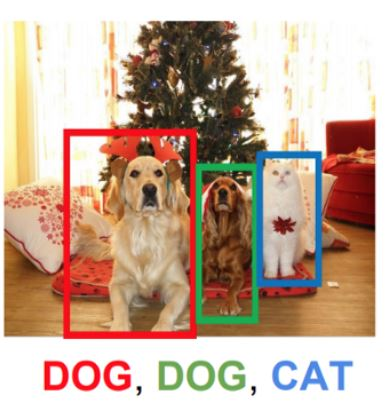
\includegraphics[width=0.3\linewidth]{notes/img/n4_image_classification.JPG} 
\hspace{2cm}
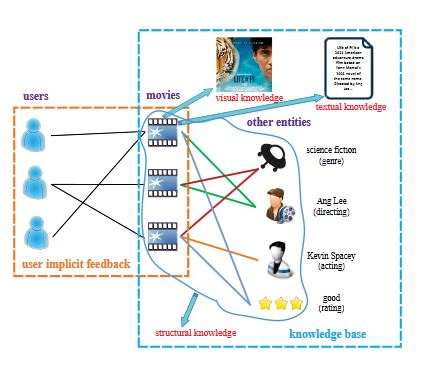
\includegraphics[width=0.4\linewidth]{notes/img/n1_movies.jpg} \par
}

This approach differs from previous influence spread/belief propagation approach. Previous methods are statistical in nature, leveraging heavily knowledge related to Bayesian networks (those that you will learn in CS228). This chapter primarily focuses on, as the section title suggest, learning a graph representation in the form of an embedding that represent graph and its components in the latent space. We will be exploring methods to generate node embedding and graph embedding in the following sections.

\subsection{Node Embedding}

Generating embedding for nodes is analogus to generating word embeddings as part of a natural language processing task. Node with similar embeddings represent similar objects, much like words with similar embeddings have similar semantic meanings. Researchers evaluate embedding similarities in L1-distance, L2-distance (or Forbenius norm), and cosine-distance. Graph applications often choose cosine distance whereas CV/NLP tasks are less biased on the selection of similarity functions.

Putting it in simple terms, we want to encode nodes so that similarity in the embedding space approximates similarity in the original network. We will be defining what \texttt{(1)} encoding function \texttt{(2)} similarity function \texttt{(3)} neighbor definition \texttt{(4)} optimization function now.

{
\centering
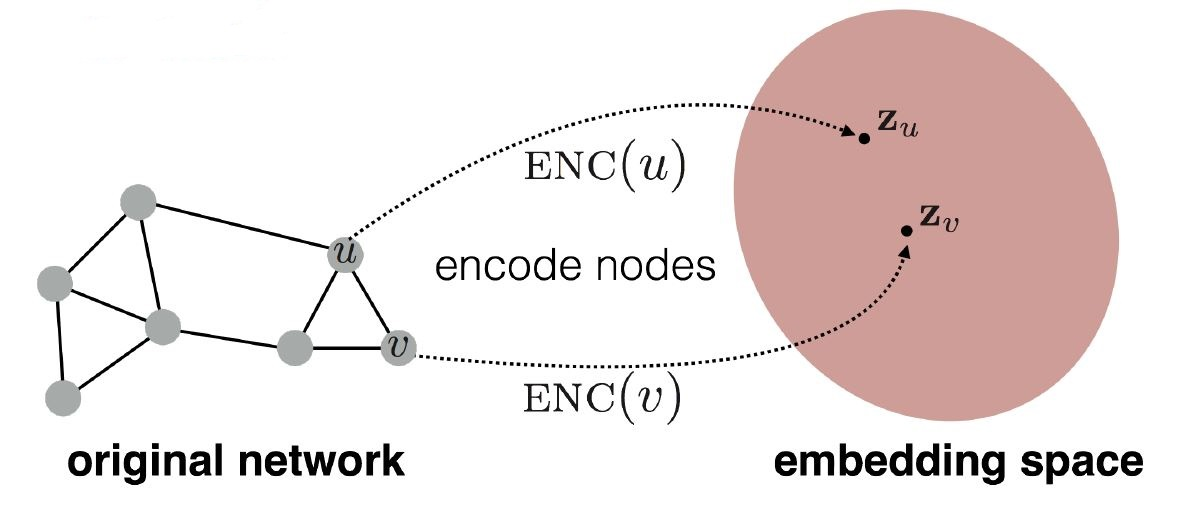
\includegraphics[width=0.65\linewidth]{notes/img/l7_p12_embedding.JPG} \par
}

\subsubsection{Some Basic Ideas}

\paragraph{Embedding lookup} is rather simple. For a graph $G(V, E)$, a node can be represented by a one-hot indicator vector $v \in \mathcal{R}^{|V|}$, and $d$-dimensional embeddings are stored in a lookup matrix $Z \in \mathcal{R}^{d \times |V|}$. Common methods to generate the embedding matrix include DeepWalk, node2vec and TransE, all of which will be covered in later sections of the note.

\begin{align}
    ENC(V_i) &= \mathbf{Z}v_i
\end{align}


\paragraph{Node similarity} can defined in a number of ways, depending on how we want to discover/evaluate node similarity. Here, we use cosine similarity to evaluate node similarity. Recall that

\begin{align}
    \vec{a} \cdot \vec{b} &= |a||b|cos(\theta)
\end{align}

Node similarity in terms of cosine similarity can simply be expressed as  the following. And of course, other similarity functions can also be employed, with appropriate change to optimization function that we will be discussing later (mostly in terms of taking derivative to minimize log-likelihood).

\begin{align}
    similarity (u, v) &= \mathbf{Z}_u \cdot \mathbf{Z}_v \\
                      &= \mathbf{Z}_u^T \mathbf{Z}_v
\end{align}{}

\subsubsection{Random Walk}\label{ss_412_rand_walk}

Here we are primarily dealing with one large graph, while the same argument applies to a number of smaller graphs as well with appropriately assigned weights to a series of smaller graphs.

Random walk is the most similar to observing sentences for a language modeling task. Imagine we convert all sentences into a large graph where graph neighbours are defined as words that are immediately next to each other, a walk along these paths should form sentence-like samples (or backwards, but backwards sentences are still useful for bi-directional recurrent models). For these language models, researchers define an \textit{n-gram} (or \textit{Skipgram}, depending on the setup) model that tracks probabilities of word co-occurance. See \href{https://web.stanford.edu/~jurafsky/slp3/3.pdf}{[here]} for Prof. Dan Jurafsky's note on \textit{N-Grams}.

{
\centering
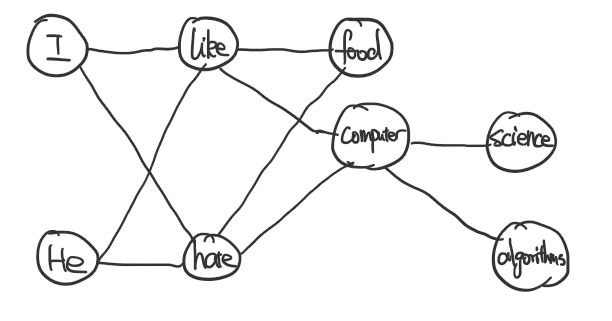
\includegraphics[width=0.65\linewidth]{notes/img/n4_sentences.JPG} \par
}

For random walk in a defined graph structure starting from node $v$, the walk consists of nodes randomly selected from neighbours of the current head. Every time a head is selected, we move to the head then use neighours of this new head as candidates for the next move. You can view this as sampling from all potential ``sentences", compared to NLP tasks where you are given many possible sentences. After sampling by random walk, similar to \textit{N-Gram}/\textit{Skipgram}, we want to find node co-occurance probabilities and match them with cosine distances between node pairs through optimizing log-likelihood.

{
\centering
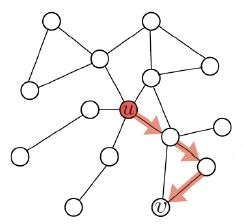
\includegraphics[width=0.4\linewidth]{notes/img/l7_p23_random_walk.JPG} \par
}

Primary benefits for random walk is the following

\begin{itemize}
    \item \textbf{Expressivity}: Walking distance and similarity function together allow incorporation of local and higher-order neighbourhood information
    
    \item \textbf{Efficiency}: Do no need to consider all node pairs and random selection is naturally weighted.
\end{itemize}{}

More formally, given graph $G=(V, E)$, embedding matrix to be optimized $\mathbf{Z} \in \mathcal{R}^{d \time |V|}$, neighbor (as defined in lecture) function $N_R(v)$ as set of nodes visited in a random walk following strategy $R$ and probability function $P$ which is really just proportional to the node similarity function. Likelihood and negative log-likelihood can be defined as the following

\begin{align}
    \mathcal{L} &= \Prod_{u \in V}P(N_R(u) | z_u) \\
    log \mathcal{L} &= \sum_{u \in V}log P(N_R(u) | z_u) \\
                    &= \sum_{u \in V}\sum_{v \in N_R(u)}log P(\mathbf{Z}_v | \mathbf{Z}_u) \\
    \intertext{\qquad \qquad Then for maximum negative log-likelihood}
                &\rightarrow \max_{\mathbf{Z}} \sum_{u \in V}\sum_{v \in N_R(u)}-log P(\mathbf{Z}_v | \mathbf{Z}_u)
    \intertext{\qquad \qquad Here, we define $P(\mathbf{Z}_v | \mathbf{Z}_u)$ as }
    P(\mathbf{Z}_v | \mathbf{Z}_u) &= \frac{exp(\mathbf{Z}_v^T\mathbf{Z}_u)}{\sum_{n \in V}exp(\mathbf{Z}_n^T\mathbf{Z}_u)} \\
    log \mathcal{L} &= \sum_{u \in V}\sum_{v \in N_R(u)}log \frac{exp(\mathbf{Z}_v^T\mathbf{Z}_u)}{\sum_{n \in V}exp(\mathbf{Z}_n^T\mathbf{Z}_u)}
\end{align}{}

We observe that denominator $\sum_{n \in V}exp(\mathbf{Z}_n^T\mathbf{Z}_u)$ have to be computed for all $v \in V$, resulting in $O(n^2)$ complexity. One way to alleviate this problem is simply sub-sample from $V$ when computing the denominator sum. We could use ``negative sampling" as used for \textit{word2vec} explained \href{https://arxiv.org/pdf/1402.3722.pdf}{[here]}. Here, ``positive" means nodes that are in $N_R(u)$ in any of the walks we performed, and ``negative" means all other nodes not visited from walks initiated from $u$. Observe the following expression. We are \texttt{(1) } maximizing $exp(\mathbf{Z}_v^T\mathbf{Z}_u)$ and minimizing sum of similarities from negative samples. ($exp$ is used here instead of $\sigma$ for sigmoid, for simplicity, the same result is achieved regardless). This way, we are minimizing the probability of a random node having high similarity with the source node. Number of negative samples (k) is typically $5-20$, depending on the application and degree of vertices in the graph. The random walks are often fixed length without preventing repeats, like \textit{DeepWalk} implementation \href{https://arxiv.org/pdf/1403.6652.pdf}{[link]}. This paper contains pseudocode and more formal work on random walk and \textit{skipgram}. For a more intuitive explanation on \textit{hierarchical softmax}, which is not immediately relevant in this context, can be found \href{https://www.quora.com/What-is-hierarchical-softmax?share=1}{[here]}.

\begin{align}
    log \frac{exp(\mathbf{Z}_v^T\mathbf{Z}_u)}{\sum_{n \in V}exp(\mathbf{Z}_n^T\mathbf{Z}_u)} &= log(exp(\mathbf{Z}_v^T\mathbf{Z}_u)) - \sum_{n \in neg\_sampling(V, walks)}exp(\mathbf{Z}_n^T\mathbf{Z}_u)
\end{align}{}

\paragraph{Biased random walk} is a random walk with a predefined node selection probability. \textit{node2vec} proposes a wal strategy that balances exploration of local neighborhood and going further out. As shown below, $S_2$ is the same ``level" as $W$, whereas $S_3$ is further out. We assign different probabilities to $S_2\ versus\ S_3, S_4$. That is, there is $\propto 2/q$ chance of going further, $\propto 1/p$ chance of returning to $S_1$ and $\propto c$ chance of going to $S_2$. (Values shown in labels need to be normalized).

{
\centering
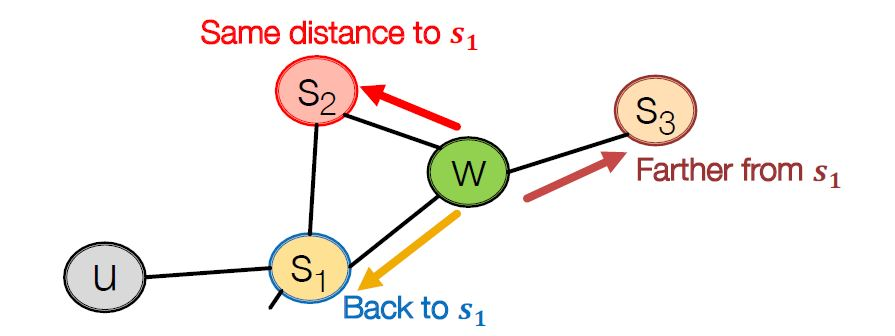
\includegraphics[width=0.45\linewidth]{notes/img/l7_p41_bias1.JPG}
\hspace{1cm}
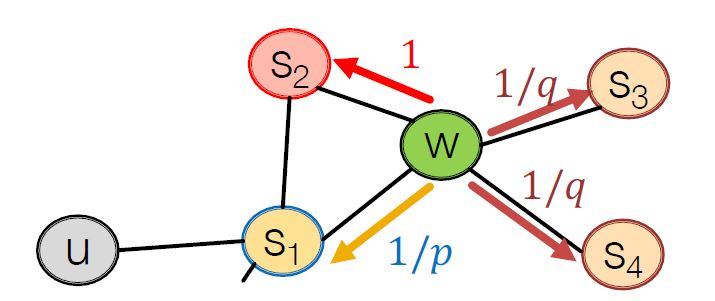
\includegraphics[width=0.45\linewidth]{notes/img/l7_p41_bias2.JPG} \par
}

This is only a different strategy of defining random walk preference ($N_R(v)$). The same gradient descent method for maximizing negative log-likelihood still applies.

We will cover \textit{TransE} later in the notes because it falls in the more ``neural" approach compared to the above more traditional approach.

\subsection{Graph Embedding} \label{ss_42_graph_emb}

Graph(sub-graph) embedding involves transforming embedding of nodes into one embedding for the entire (sub)graph. Typical embedding `joint" methods include 

\begin{itemize}
    \item Concatenation
    
    \item Hadamard (element-wise product)
    
    \item Sum/Avg (element-wise sum/average)
    
    \item Distance (distance between embeddings with some distance function suitable for $2$ or more vectors)
\end{itemize}{}

There are clearly more effective methods than the above embedding joining methods that lead to higher quality graph-level embeddings.

\subsubsection{Naive Concatenation}

As said, we just naively run some node embedding algorithm (neural or traditional), then average all node embeddings \href{https://arxiv.org/pdf/1509.09292.pdf}{[link]}. This is the most robust as embeddings will have fixed length and not blow up/vanish in scale if sum or product is taken. 

\subsubsection{Virtual Node}

Instead of averaging embeddings, we create a virtual node that connects to the entire graph (or relevant nodes only, for sub-graph) then compute embedding for the virtual node. Analogy of this is creating a source/sink pair when we are transforming difficult graph problems to max flow min cut problems that have well-known fast-ish solution. See the publication \href{https://arxiv.org/abs/1511.05493}{[here]}.

\subsubsection{Anonymous Walk}

Anonymous walk is a fancy name of saying instead of having a $|V|$ size one-hot vector, we only use a size $k$ one-hot vector for a $k$-length random walk. That is, we only care about whether a different node has been visited in a walk, rather than the actual identity of the node. 

{
\centering
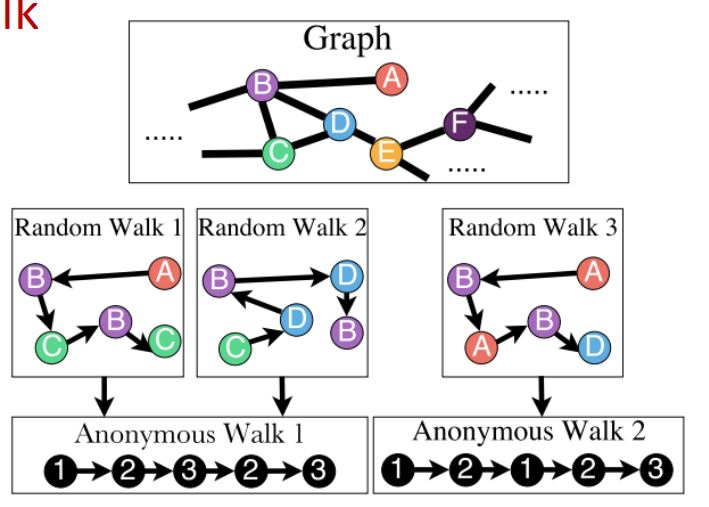
\includegraphics[width=0.55\linewidth]{notes/img/l7_p58_anonymous.JPG} \par
}

As expected, total number of different $k$-length grows as $k$ increases. In fact, it should grow proportionally (but faster than) to $\frac{k^k}{p!}$ (think about how many, allowing repeats, different combinations can exist). This estimate is NOT accurate because it over-penalizes low $k$ scenarios. The growth chart below reflect the true number of anonymous walks. The approximation ratio grows (or shrinks, depends on how you define approximation ratio) at approximately $2$.

{
\centering
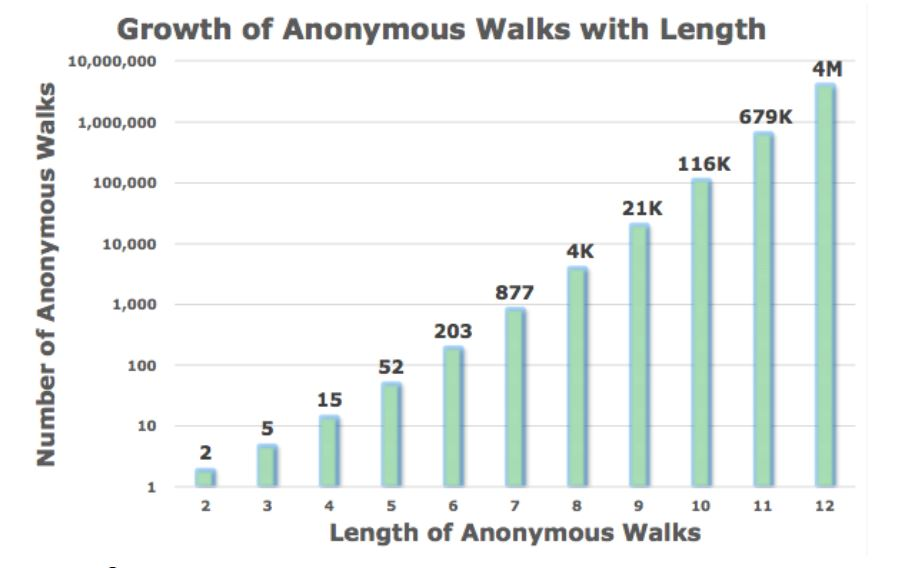
\includegraphics[width=0.55\linewidth]{notes/img/l7_p59_count.JPG} \par
}

\paragraph{Idea 1, enumerate all walks} We define $d$ as number of distinct random walks for length-$k$ walks. Then each $\mathbf{Z}_v^{i}$ is the probability of obtaining the i-th anonymous walk starting the walk at node $v$. Without considering weight associated with bias, we can enumerate all possible walk paths then for each node, we compute the probability of obtaining the $i$-th anonymous walk starting at node $v$.

\paragraph{Idea 2, sample and deal with sampling error} We can obtain the previous probability by sampling a large number of random walks then process for each node. Here we use some statistical trick to argue that to obtain error of no more than $\epsilon$ with probability less than $\delta$, we need to sample

\begin{align}
    m = \Big[\frac{2}{\epsilon^2}(log(2^\eta - 2) - log(\delta))\Big] \comment{where\ $\eta$ is number of different anonymous walks for $k$-length walk}
\end{align}{}

\begin{todo}
    I suspect this is derived from multiplicative form of Chernoff bound. Wikipedia page for Chernoff bound is not a bad place to start \href{https://en.wikipedia.org/wiki/Chernoff_bound}{[link]}.
\end{todo}{}

\paragraph{Idea 3, use Skipgram again} Notice that the above ``dumb" methods are what NLP researchers used to create language model. \textbf{Idea 2} is not much different for the argument that negative sampling reaches approximately the same error, if you spent the time of digging all the formalities out. Therefore, \textbf{Idea 3} is simply treat each anonymous walk as a ``token". Suppose from node $v$ we can have anonymous walks $w_1, w_2 \dots w_t$, then as defined for \textit{Skipgram}, we want to maximize $P(w_m | \{w_1, w_2 \dots w_t\} \setminus w_m)$. We are claiming that $N_R(u) = \{w_1, w_2 \dots w_t\}$, re-using the neighborhood notation we user earlier for node embedding. All other expressions for \textit{Skipgram} applies and we want to maximize, as in lecture

\begin{align}
    max \frac{1}{T}\sum_{t=\delta}^{T}log P(w_t|w_{t-\delta}, \dots w_{t-1})\\
    P(w_t|w_{t-\delta}, \dots w_{t-1}) &= \frac{exp(y(w_t))}{\sum_i^{\eta} exp(y(w_i))} \\
    y(w_t) &= b + U \cdot (\frac{1}{\delta}\sum_{i=1}^{\delta}v_i)
\end{align}{}

Formal derivation of this part of the notes is discussed in the \textit{Anonymous Walk Embedding} paper \href{https://arxiv.org/pdf/1805.11921.pdf}{[link]}.


\section{Convolutional Model for Graphs}

In the previous section, we discussed traditional methods of generating embeddings for node and graphs. In this section, we move on to neural models that started gaining tracking only in recent years (approximately 2013, when the foundational \textit{TransE} paper was published \href{https://papers.nips.cc/paper/5071-translating-embeddings-for-modeling-multi-relational-data.pdf}{[link]}). This progress, viewing it from the perspective of Stanford's AI course offerings, is from CS229 (machine learning) to CS230 (deep learning). In terms of actual methods used, we are moving from \textit{word2vec} and \textit{Skipgram} model to convolutional and recurrent neural networks. For graph related topics, the following content is the neural ``equivalent" for CS228 (probabilistic graphical models).

There are several problems with getting embedding from random walks as shown in Section \ref{ss_4_graph_repr}. \texttt{(1)} these node embeddings are generated independently (at best locally) from each other (remember that we are only approximating the log-likelihood) \texttt{(2)} we cannot generate node embedding for future nodes, which means the graph itself is pre-determined, \texttt{(3)} the incorporation of local/macro level structure is questionable despite us playing with biased random walk while leaving structure of the graph itself on the table.

Applying existing models like convolutional neural network and recurrent neural network sounds problematic because they are designed for samples that has internal structures, not samples that are well-structured (but not following a fixed pattern) to connect to other samples. For example, in the case of image convolution, we define a $d_1 \times d_2 \times c$ (dim, dim, channel) kernel that scans the image. This is clearly not possible as we cannot define a fixed size ``kernel" for graphs because nodes do not all have the same edge connectivities. 

{
\centering
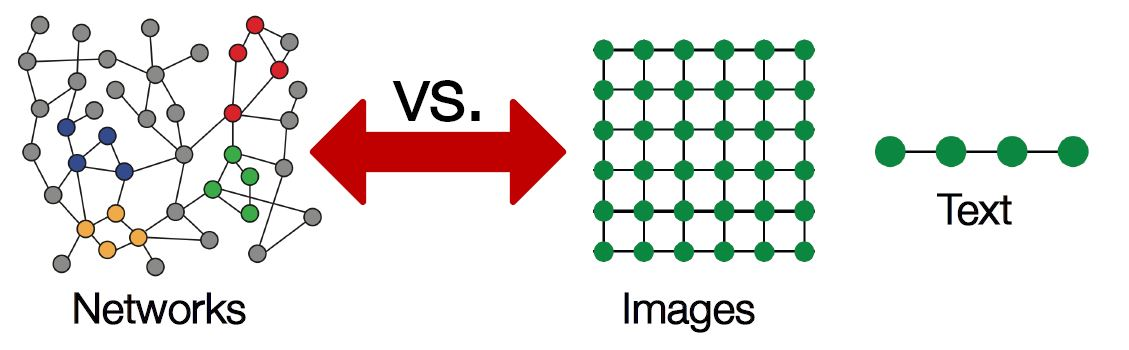
\includegraphics[width=0.75\linewidth]{notes/img/l8_p12_compare.JPG} \par
}

\subsection{Components of Graph Convolution}

Naturally, convolution is a form of recursion where recursion depth is number of layers we include in the convolution. To fully define this ``recursion" we need to figure out \texttt{(1)} what do to with embedding from previous layer? \texttt{(2)} what message is passed from node in the previous layer to the current node \texttt{(3)} how to aggregate messages from previous layer \texttt{(4)} how to aggregate/post-process this aggregated message with embedding of the current node. Putting everything together, for $h_v^k$ as embedding for node $v$ after $k$-th recursion,

\begin{align}
    h_v^k &= \phi(AGG_1\Big[ op_1\big[(AGG_2(\{MSG(u, v), \forall u\in N(v)\})\big], op_2(h_v^{k-1})  \Big])
\end{align}{}

We define the various ``placeholder functions" as the following. I'm sure you can also convert computer vision task to something like this where $h_v^k$ is equivalent to a pixel-level multi-channel vector. 

\begin{itemize}
    \item $\phi \rightarrow$ Activation function for embedding (tanh, softmax, etc.)
    
    \item $AGG_1 \rightarrow$ Aggregation function to join embedding from previous layers and embedding of current node from previous step (concatenation, sum/avg, attention, etc.)
    
    \item $op_1 \rightarrow$ Weight assigned to messages from previous layer after aggregation (typically just a matrix multiply)
    
    \item $AGG_2 \rightarrow$ Aggregation function to join embedding from nodes in the previous layer(concatenation, sum/avg, attention, etc.)
    
    \item $AGG_2 \rightarrow$ Message function to compute message from nodes in the previous layer to current node (depends on whether edge embeddings exist or if we are handling non-existing edges differently)
    
    \item $op_2 \rightarrow$ Weight assigned to embedding of the current node from previous iteration (typically just a matrix multiply)
    
    \item $N \rightarrow$ Neighbour of a node (typically immediate neighbours, but researchers have used other definitions, such as \textit{RippleNet}, \href{https://arxiv.org/pdf/1803.03467.pdf}{[link]})
\end{itemize}

On top of this, of course, there is also embedding initialization methods and loss function for gradient descent. Little generalization can be applied to these functions as they are task dependent.

A comprehensive survey of various graph neural network methods as of 2019 is \href{https://arxiv.org/pdf/1901.00596.pdf}{[here]} and \href{https://arxiv.org/pdf/1812.08434.pdf}{[here, a bit older]}. For this class, we discuss \textit{TransE} (Sec \ref{ss_52_transe}), \textit{Trans[OTHERS]} (Sec \ref{ss_53_transr}), \textit{GraphSAGE} (Sec \ref{ss_54_sage}), \textit{PinSage} (Sec \ref{ss_55_pin_sage}) and \textit{GAT} (Sec \ref{ss_56_gat}). We could argue that the various Trans[X] models are not exactly neural. However, we can think of them as neural methods that have nothing to do with the graph structure, but only contain a minor manipulation (a simple layer) on node/edge embedding then a loss function. Note that neural methods can still share the same loss function as those defined as these Trans[X] methods.


\subsection{TransE, Translating Embeddings for Modeling Multi-relational Data} \label{ss_52_transe}

The foundational TransE implementation was proposed in 2013 \href{https://everest.hds.utc.fr/lib/exe/fetch.php?media=en:cr_paper_nips13.pdf}{[link]}. We reproduce the algorithm (not a screenshot) below. We define $(h, l ,t)$ triplet as (head entity, relation, tail entity), or graphically, $v_h \xrightarrow[]{l} t_h$. For distance function, the authors defined $d(h+l, t)= h + l -t$. 

\begin{algorithm}[H]
\SetAlgoLined
%\KwResult{Write here the result }
\textbf{input:} Training set $S=\{h, l, t\}$, entities and rel.sets $E$ and $L$, margin $\gamma$, embeddings dim. $k$. \\
%\hspace*{\algorithmicindent} \textbf{Input:}\\
%\hspace*{\algorithmicindent} \textbf{Output} 
\textbf{initialization} \\
\hspace*{\algorithmicindent} $l = uniform(-\frac{6}{\sqrt{k}}, -\frac{6}{\sqrt{k}}) \qquad  \forall l \in L$ \Comment{$\frac{6}{\sqrt{k}}$ is most likely from Xavier initialization} \\
\hspace*{\algorithmicindent} $l = l / ||l|| \qquad \forall l \in L$ \\
\hspace*{\algorithmicindent} $e = uniform(-\frac{6}{\sqrt{k}}, -\frac{6}{\sqrt{k}}) \qquad \forall e \in E$ \\
\While{Loss not converged}{
    $e = e / ||e|| \qquad \forall e \in E$ \\
    $S_{batch} = rand\_sample(S, b)$ \Comment{sample $b$ triplets from set $S$} \\
    $T_{batch} = \emptyset$ \Comment{Set initial pairs of triplets to be empty} \\
    \For{$(h, l, t) \in S_batch$}{
      $(h', l, t') = rand\_sample(S')$ \Comment{Sample an invalid $(h', l, t')$ triplet (exactly one or two of $h, l, t$ have to be different)} \\
      $T_{batch} = T_{batch} \cup \{((h, l, t), (h', l, t'))\}$
     }
 Gradient descent on $\sum_{((h, l, t), (h', l, t')) \in T_{batch}} \nabla[\gamma + d(h + l, t) - d(h' + l, t')]$
 \caption{Learning \textbf{TransE}}
 }
\end{algorithm}

To explain what this ``sample an invalid triplet" is all about, let's use a visual Q\&A example \href{https://people.cs.vt.edu/sudo777/files/siamese-network-pptx.pdf}{[link]}. With this example, you want to make sure that embedding of an image with \underline{girl} \textit{walking a bike} is different from images \underline{boy} \textit{walking a bike}. So, $h$ is \textit{boy/girl}, $l$ is \textit{walking a bike}, $t$ is the image. We want to make sure that translating \textit{boy/girl} with operator \textit{walking a bike} do NOT land in the same target image. Hopefully this analogy help you understand the rationale behind setting up the gradient update rule. Search for \texit{Siamese network} \href{https://en.wikipedia.org/wiki/Siamese_neural_network}{[link]} for similar setups (commonly used for facial identification).

{
\centering
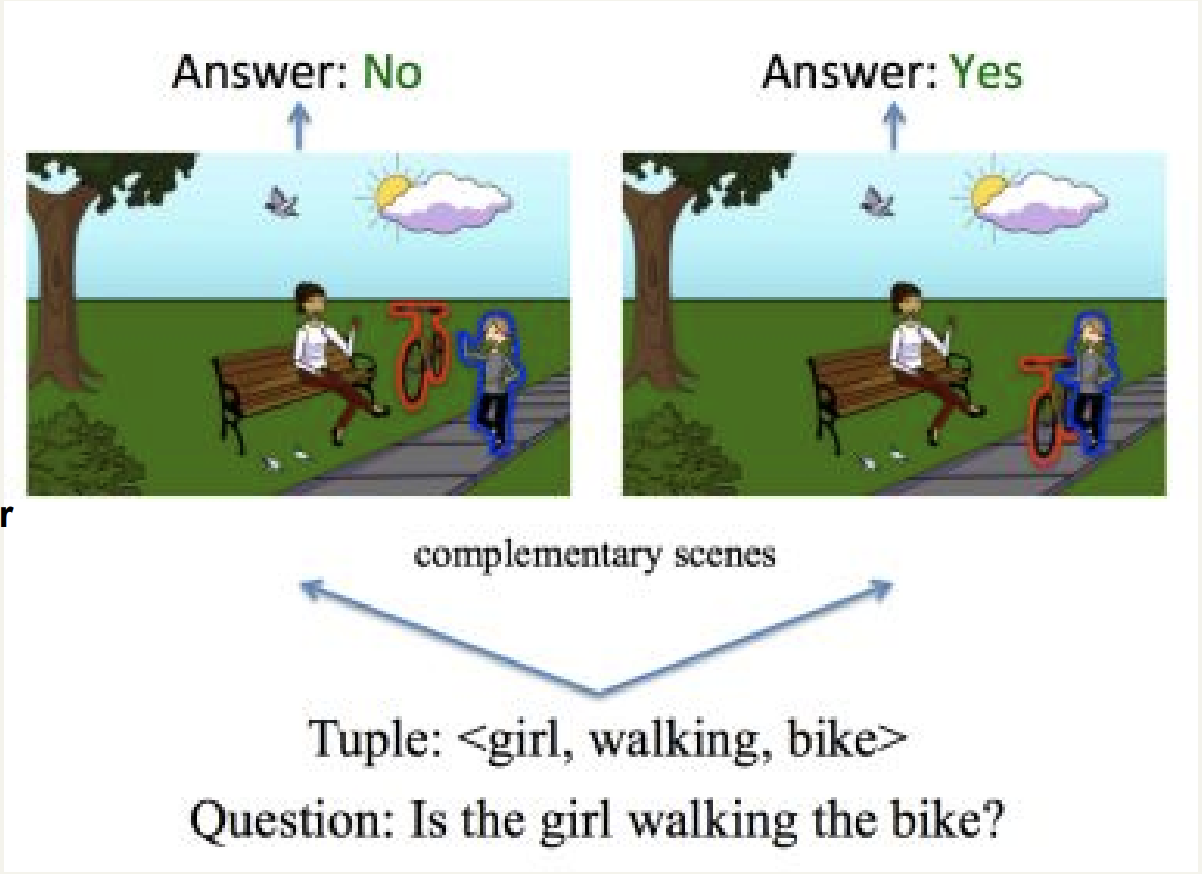
\includegraphics[width=0.6\linewidth]{notes/img/n5_siamese.png} \par
}

\subsection{Many other Trans[X] models} \label{ss_53_transr}

Numerous Trans[X] have been proposed following the success of TransE. A collection of these models and cmparison of performance is presented \href{https://github.com/thunlp/KB2E}{[here]}.

\paragraph{TransH} Knowledge Graph Embedding by Translating on Hyperplanes (AAAI 2014) \href{https://www.aaai.org/ocs/index.php/AAAI/AAAI14/paper/viewFile/8531/8546}{[link]}. This model claims to better handle reflexive (think of ``invertible"), many-to-one and one-to-many relationships by projecting $h, t$ onto a hyperplane first before training using TransE metrics. That is, for each relationship $r$, we derive a hyperplane represented by $w_r$. Then the distance function becomes $d(h+r, t) = ||(h - w_r^Thw_r) + r - (t - w_r^Ttw_r)||_2$. Notice that the additional vector means all relationships now require one additional $\mathcal{R}^k$ vector, increasing model complexity. Image below shows TransH projecting both $h$ and $r$ onto the same hyperplane first before computing distance measure. 

{
\centering
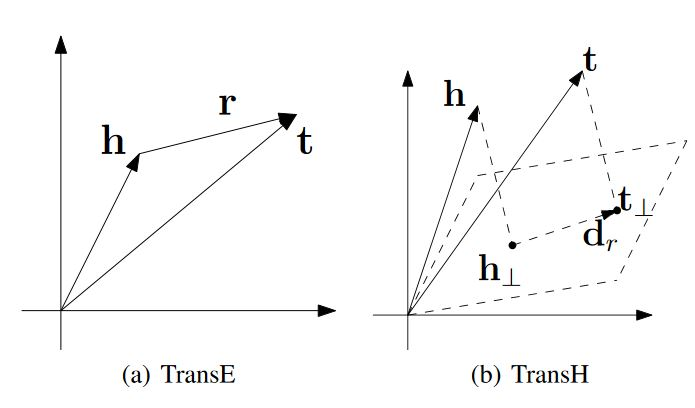
\includegraphics[width=0.5\linewidth]{notes/img/n5_transh.JPG} \par
}

\paragraph{TransR} Learning Entity and Relation Embeddings for Knowledge Graph Completion (AAAI 2015) \href{https://www.aaai.org/ocs/index.php/AAAI/AAAI15/paper/viewFile/9571/9523}{[link]}. The main argument for TransR is that node embeddings can be in distinct entity space for different relationships. TransE and TransH assumed that all embeddings exist in one shared latent space. As you might have guessed, the new distance function is simply $d(h+r, t) = ||hM_r + r - tM_r||_2$ with translation matrix $M_r$ for each relation $r$. Notice how this is the same thing as applying a $1-layer$ perceptron to node embeddings (and remember this fact if you want to implement this method).

In lecture you saw this image as part of TransE, but it should be part of TransR.

{
\centering
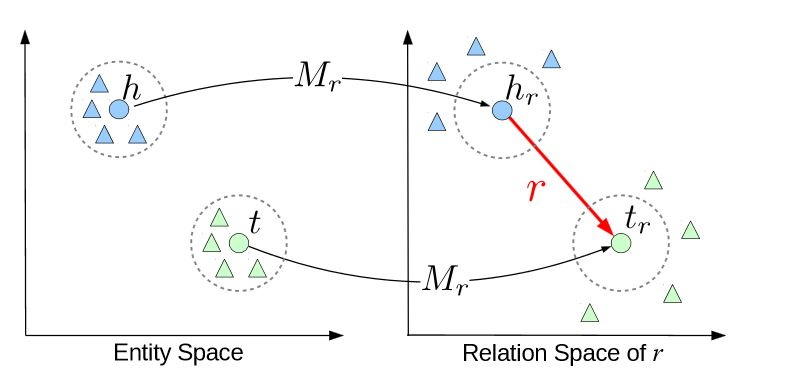
\includegraphics[width=0.5\linewidth]{notes/img/n5_transr.JPG} \par
}

\paragraph{TransD} Knowledge Graph Embedding via Dynamic Mapping Matrix (ACL 2015) \href{https://www.aclweb.org/anthology/P15-1067.pdf}{[link]}. This work goes one step further than TranR, arguing that all entities and relations require individual projections, therefore, we have to create projection vector $v_p$ (turns into $h_p, t_p$ for equation) and $r_p$. We then have 

\begin{align}
    M_{rh} &= r_p h_p^T + I^{m \times n} \\
    M_{rt} &= r_p t_p^T + I^{m \times n} \\
    h_{\perp} &= M_{rh}h \\
    t_{\perp} &= M_{rt}t \\
    d(h+r, t) &= ||h_{\perp} + r - t_{\perp}||_2
\end{align}{}

Notice that $M_{rh}, M_{rt}$ look suspiciously like a neuron with bias. Again, these Trans[X] methods only deal with embedding, but we can look at them from a neural lens and stuff them into frameworks like Tensorflow and Pytorch.

Each of the papers we referenced here have a well-written (though the same content) background section and performance/model compelxity comparison against previous models. Read the original papers to compare number of parameters needed for each of these models.

\subsection{Vanilla Graph Convolution}

We have developed a very general version of what all graph convolution methods should look like. A vanilla graph convolutional neural network defines node embedding as 

\begin{align}
    h_v^k &= \sigma\Big( W_k \sum_{u \in N(v)} \frac{h_u^{k-1}}{|N(v)|} + B_kh_v^{k-1} \Big)
\end{align}{}

Here, $\sigma$ is an activation function like \textit{ReLU} or \textit{Tanh}. $W_k \sum_{u \in N(v)} \frac{h_u^{k-1}}{|N(v)|}$ gives a transformed average embedding from neighbours, $B_kh_v^{k-1}$ gives a transformed embedding from previous iteration. Hence aggregation is just taking average, and the \textit{op} is simple matrix multiplication.

In fully vectorized form, for embedding matrix $H=[h_1, h_2, \dots h_{|v|}]$, $A$ as adjacency matrix, $D$ as degree matrix, and $\hat{A}=D^{-1/2}AD^{-1/2}$

\begin{align}
    H^{(l+1)} &= \sigma(H^{(l)}W_0^{(l)} + \hat{A}H^{(l)}W_1^{(l)})
\end{align}{}

After obtaining the embeddings, we can \texttt{(1)} Use one of the Trans[X] methods to further manipulate the embeddings and leverage its loss function \texttt{(2)} Directly use it for prediction by passing it through $1$ additional neural layer for $n$-class classification \texttt{(3)} Dot-product (or any distance metric) with nodes that should be in the same class with appropriate loss aggregation. All of these lead to an aggregate loss from which gradient descent method can be used to optimize embeddings. Most graph neural networks follow the same setup.

\subsection{GraphSAGE, Inductive Representation Learning on Large Graphs} \label{ss_54_sage}

GraphSAGE (NIPS 2017) \href{https://arxiv.org/pdf/1706.02216.pdf}{[link]} does \texttt{(1)} replaces taking average with a generic aggregation function \texttt{(2)} replaces embedding addition with embedding concatenation. Its expression can be written as 

\begin{align}
    h_v^k &= \sigma\Big( CONCAT[AGG(h_u^{k-1}, \forall u \in N(v)), B_kh_v^{k-1} ]\Big)
\end{align}{}

Here, the generalize aggregation function can be average, max pool, min pool, RNN or any method that converts a collection of neighbour embeddings into one aggregate embedding.

\subsection{PinSage, Graph Convolutional Neural Networks for Web-Scale Recommender Systems} \label{ss_55_pin_sage}

Pinsage (KDD 2018) \href{https://arxiv.org/pdf/1806.01973.pdf}{[link]} is an improvement on GraphSAGE, making it suitable for processing large graphs. Remember that Pinterest has billions of images and many more interconnecting edges. It is impossible to perform matrix multiplications that we came up with just now. Instead of aggregating on all neighbours, Pinsage samples a select set of neighbours then perform aggregation on these neighbours only. 

The Pinsage formulation is a bit more involved, so we break it down to a few steps. The first is convolution step, $Q, W$ are weight matrices, $q, w$ are bias, $\alpha$ is a scaling factor. Notice that we are multiplying all neighbours by a shared weight then scaled by neighbour importance function $\alpha$. Then the normal GraphSAGE-like aggregation with bias is applied. Finally new embedding is normalized to ensure its magnitute does not change over several iterations.

\begin{align}
    n_u &= \sigma\Big(\alpha[ReLU(Qh_v + q), \forall v in N(u)]\Big) \\
    h_u^{new} &= ReLU(W \cdot CONCAT(h_u, n_u) + w) \\
    h_u^{new} &= \frac{h_u^{new}}{||h_u^{new}||_2}
\end{align}{}

Neighbourhood definition is fairly simple. Again we have neighbourhood function $N(u)$ for vertex $u$. At layer $1$, neighbours are simply $N(u)$, but in the second layer, we have to perform convolution on $N(u) \cup u$, the third layer is consequently $N(N(u)) \cup N(u) \cup u$. You can think of this as a wave propagating outward where the center is still generating new waves. The same analogy is applicable to vanilla GCN.

From the paper, these neighbourhoods are sub-sampled based on visit frequency (by tracking set union with counts) to reduce total number of neighbours involved in the convolution. Also, node mini-batches with positive and negative samples are selected such that only a small portion of the graph need to be loaded at a time. The graph is re-indexed to so that a generic graph neural network algorithm can still process the adjacency matrix. This concept is seen in numerous other GNN implementations. In fact, extracting a sub-graph is relatively easy for Pinterest because as described before, the Pinterest graph only has $3$ components: images, boards and users.

\subsection{GAT, Graph Attention Networks} \label{ss_56_gat}

In PinSAGE we introduced a neighbour importance parameter $\alpha$. This parameter originates from Graph Attention Network (ICLR 2018) \href{https://arxiv.org/pdf/1710.10903.pdf}{[link]}. The effect of graph attention is similar to attention for NLP tasks, where the model learns to ignore certain neighbours that have low priority, like skipping \textit{and, a, the}, etc. for developing semantic understanding. We can also have multi-head attention the same way as NLP ones, which we won't be discussing in this note. The image below represents how \texttt{(1)} attention weight is computed between $2$ nodes \texttt{(2)} how attentions are used together to re-weight neighbour contributions.

{
\centering
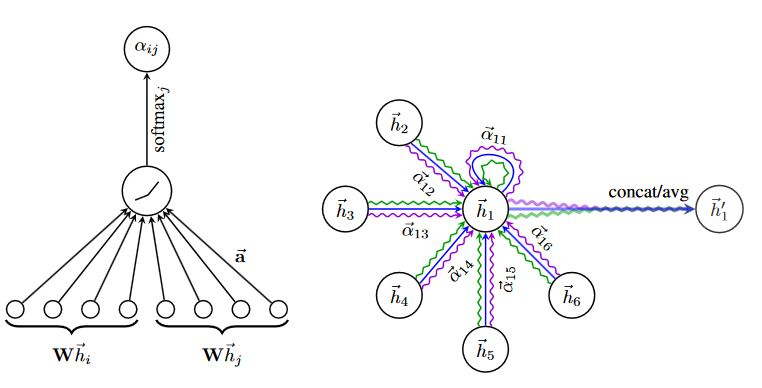
\includegraphics[width=0.75\linewidth]{notes/img/n5_gat.JPG} \par
}

Define $\alpha$ as a function that describes such importance assignment function, then attention coefficients $e_{v \rightarrow u}$ can be written as 

\begin{align}
    e_{vu} &= \alpha(Wh_u, W_h_v) \\
    \intertext{\qquad \qquad Consequently, we can write $\alpha_{vu}$}
    \alpha_{vu} &= softmax_i(e_{vu}) \\
                &= \frac{e_{vu}}{\sum_{q \in N(u)}e_{qu}}
\end{align}{}

In the original GAT implementation, attention mechanism $\alpha$ was implemented as a $1$-layer neural network with LeakyReLU activation scaled by $\hat{\alpha}$ (for a $1$-layer neural network, its parameters should be a matrix, but we only have a scaler output, thus $\hat{\alpha}$ is sufficient). We can re-write the above $e_{vu}$ as 

\begin{align}
    e_{vu} &= \hat{\alpha} \cdot CONCAT[Wh_u, Wh_v]
\end{align}{}

Then finally we can express node embedding $h_u$ as 

\begin{align}
    h_u^{new} &= \sigma\Big(\sum_{v \in N(u)}a_{vu}Wh_v\Big)
\end{align}{}

\subsection{List of other notable papers}

See a list of notable papers \href{https://snap-stanford.github.io/cs224w-notes/machine-learning-with-networks/graph-neural-networks}{[here]}.

%The following is a list of papers listed in lecture.

%\begin{enumerate}{}
 %   \item Relational inductive biases, deep learning and graph networks (Battaglia et al., 2018) \href{https://arxiv.org/pdf/1806.01261.pdf}{[link]}

  %  \item Representation learning on graphs: Methods and applications (Hamilton et al., 2017) \href{https://arxiv.org/pdf/1709.05584.pdf}{[link]}
    
   % \item Graph attention networks (Hoshen, 2017 \href{https://papers.nips.cc/paper/6863-vain-attentional-multi-agent-predictive-modeling.pdf}{[link]}; Velickovic et al., 2018 \href{https://arxiv.org/pdf/1710.10903.pdf}{[link]}; Liu et al., 2018 \href{?}{[link]})
    
    %\item Graph neural nets with edge embeddings (Battaglia et al., 2016 \href{nteraction networks for learning aboutobjects, relations and physics}{[link]}; Gilmer et. al., 2017 \href{https://dl.acm.org/ft_gateway.cfm?id=3305512&type=pdf}{[link]})
    
    %\item Embedding entire graphs (Duvenaud et al., 2015 \href{https://papers.nips.cc/paper/5954-convolutional-networks-on-graphs-for-learning-molecular-fingerprints.pdf}{[link]}; Dai et al., 2016 \href{http://proceedings.mlr.press/v48/daib16.pdf}{[link]}; Li et al., 2018 \href{??}{[link]}) and graph pooling
%(Ying et al., 2018 \href{https://papers.nips.cc/paper/7729-hierarchical-graph-representation-learning-with-differentiable-pooling.pdf}{[link]}, Zhang et al., 2018 \href{https://www.aaai.org/ocs/index.php/AAAI/AAAI18/paper/download/17146/16755}{[link]})
    
 %   \item Graph generation and relational inference (You et al., 2018 \href{}{[link]}; Kipf et al., 2018 \href{https://arxiv.org/pdf/1802.04687.pdf}{[link]})
    
  %  \item Varying neighborhood: Jumping knowledge networks (Xu et al., 2018 \href{}{[link]}), GeniePath (Liu et al., 2018 \href{}{[link]})
    
   % \item Position-aware GNN (You et al. 2019 \href{}{[link]})
    
    %\item Spectral graph CNN & ChebNet (Bruna et al., 2015 \href{}{[link]}; Defferrard et al., 2016 \href{}{[link]})
    
    %\item Geometric deep learning (Bronstein et al., 2017 \href{}{[link]}; Monti et al., 2017 \href{}{[link]}) 
    
    %\item Pre-training Graph Neural Networks (Hu et al., 2019) \href{}{[link]}
    
   % \item GNNExplainer: Generating Explanations for Graph Neural Networks (Ying et al., 2019) \href{}{[link]}
%\end{enumerate}

\section{Recurrent Model for Graphs}

The previous section built the foundation for applying neural methods for graph problems. We covered a number of Trans[X] models and convolutional models. Here, we continue on to recurrent model for graphs. We do not make the distinction between LSTM and GRU, as suitable recurrent models can be easily swapped, as long as dependencies (for generative models) are respected. 

See class note of CS224N on general recurrent structures \href{https://web.stanford.edu/class/archive/cs/cs224n/cs224n.1194/readings/cs224n-2019-notes05-LM_RNN.pdf}{[link]}.

\subsection{Recurrent Model for Graph Embedding}

Recall that in Section \label{ss_412_rand_walk} and Section \label{ss_42_graph_emb} we discussed how to use random walk and similarity function to represent transition probabilities of such random walk. Instead of computing $P(x_t | x_{t-1} \dots x_1)$ for co-occurance probability, we pass the corresponding embeddings $h_1 \dots h_t$ to LSTM model. One such implementation is presented in Learning Graph-Level Representations withRecurrent Neural Networks \href{https://arxiv.org/pdf/1805.07683.pdf}{[link]}, presented as below. Notice that the model has additional input channel $Nb_t$, meaning that it takes both \texttt{(1)} embedding of node on the walk $e_t$ AND \texttt{(2)} aggregated node information from $N(t) \rightarrow Nb(t)$. 

Author of this paper acknowledge the issue of random walk with graph isomorphism. With sufficient number of walks sampled and having an order-invariant aggregation function (sum, average, max-pool) make it at least independent of order of aggregation. We should be mindful of inherent property of data before deciding on the operator (associative vs non-associative, proper way of saying order-invariant). For example, chirality is quite important for classifying molecular properties, hence non-associate aggergators should be used. Note that the same walk embedding $\rightarrow$ graph embedding procedure still applies here as they did in Section \label{ss_412_rand_walk} and \label{ss_42_graph_emb}.

{
\centering
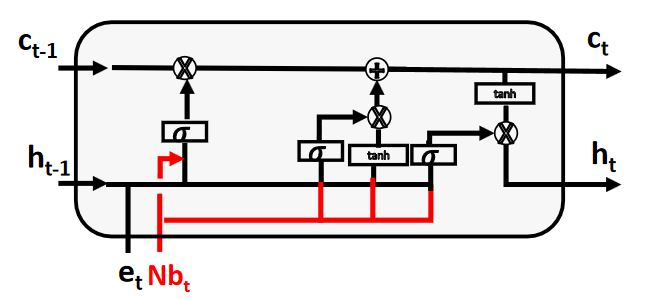
\includegraphics[width=0.7\linewidth]{notes/img/n6_lstm.JPG} \par
}

\subsection{Recurrent Model for Graph Generation}

Graph generation is useful for \texttt{(1)} anomaly detection (abnormal behavior, evolution) \texttt{(2)} prediction (predicting future from the past) \texttt{(3)} simulation (simulation of graph structures) \texttt{(4)} graph completion (many graphs are partially observed) \texttt{(5)} ``what if " scenarios \texttt{(6)} insight into the graph formation process itself. Just like any generative model, the generated graph either has to be realistic 
(social network), or satisfies a certain criteria (drug discovery), or both.

\subsubsection{Basics of Generative Models} \label{ss_621_basics}

Any generative problem is hard because the typical setup is generating a large output from limited input. For example, image generation models start with a random vector and outputs a meaningful image. Graph generation problems are typically given a set of known nodes (a number of atoms available for drug molecule) and the output is connection between these nodes. Essentially generating a $n \times n$ adjacency matrix from $n$ nodes. As discussed before, there are also isomorphic graphs that we might have to identify/resolve given properties of the problem. Image below shows that isomorphic graphs can have very different adjacency matrices. Unlike images where pixels are locally correlated and larger features are globally correlated, each edge in a graph can depend on the entire graph due to \textit{long range dependencies}. 

{
\centering
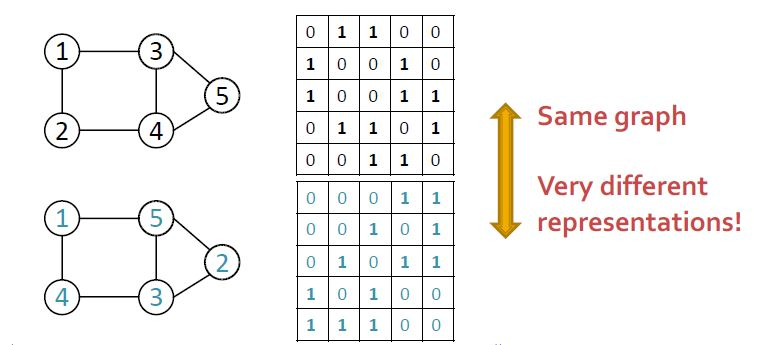
\includegraphics[width=0.7\linewidth]{notes/img/l10_p19_isomorphism.JPG} \par
}

We should be familiar with the probabilistic interpretation of generative model. Suppose we have data $(X, Y)$ where $X$ is data, $Y$ is label and $\theta$ is the set of model parameters.

\begin{itemize}
    \item \textbf{Discriminative} Find $\theta$ to maximize $P(Y=y|X, \theta)$
    
    \item \textbf{Generative} Find $\theta$ to maximize $P(X|Y=y, \theta)$
    
    \item \textbf{Generative (without class label)} Find $\theta$ to maximize $P(X, \theta)$
\end{itemize}

Expressing the without class label case for the entire dataset, then we want to have MLE parameter $\theta^{*}$

\begin{align}
    \theta^{*} &= \argmax_{\theta} \sum_{x_i \in X} log P(x_i|\theta)
\end{align}{}

And for generating the actual sample, we simply apply the with class label case and find $x_{gen}$ that maximizes $P(x_i|y, \theta)$. For sequential generators, we express the total generated probability as the following, where $t$ represent one sample generation step.

\begin{align}
    P(\mathbf{x}; \theta) = \prod_{t=1}^{n}P(x_t|x_{t-1}, \dots x_1; \theta)
\end{align}{}

This can of course be tackled using traditional Bayesian methods, as those presented in CS228. An lineage of generative models is presented below as part of Ian Goodfellow's 2016 paper on GAN \href{https://arxiv.org/pdf/1701.00160.pdf}{[link]}. GSN here stands for generative stochastic network, first presented \href{https://arxiv.org/pdf/1503.05571.pdf}{[here]}, serving as a generalized denoising auto-encoder.

{
\centering
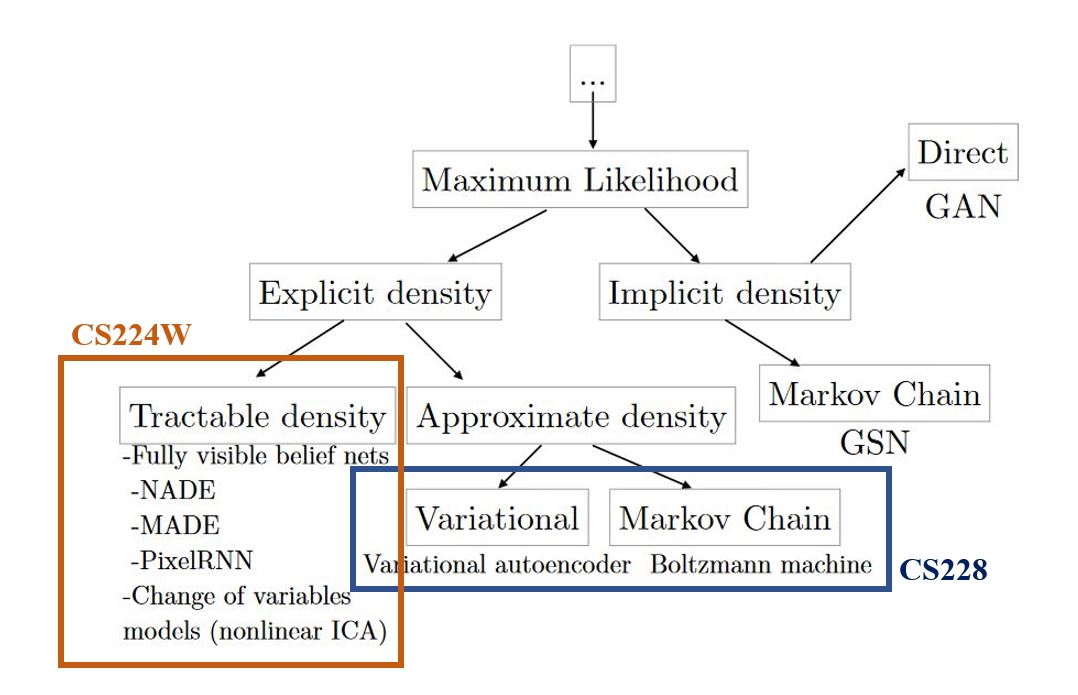
\includegraphics[width=0.85\linewidth]{notes/img/n6_gen_models_2.JPG} \par
}

The models we discuss here for graph generation serves both density estimation and sampling. This is different from GAN and VAE (variational auto-encoder) where a distinct generator-discriminator separation is built in.

\subsubsection{Graph RNN}

GraphRNN was proposed in 2018 \href{https://cs.stanford.edu/~jure/pubs/graphrnn-icml18.pdf}{[link]} to tackle the issue of graph generation using neural methods. Instead of generating all images at once, we treat graph generation as a sequential problem. That is \texttt{(1)} At the beginning, start with $1$ node \texttt{(2)} For each subsequent step, add $1$ additional node, then decide whether edges exist between this added node with all existing nodes.

{
\centering
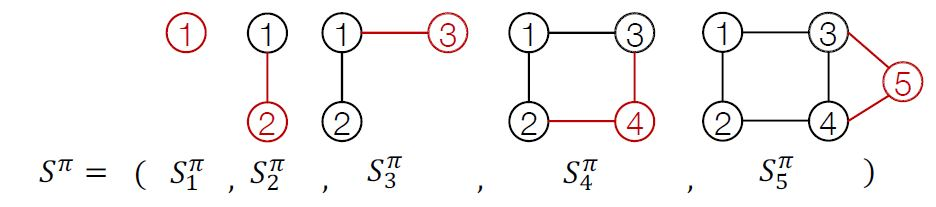
\includegraphics[width=0.85\linewidth]{notes/img/l10_p32_graph_gen.JPG} \par
}

In the above illustration, $S_{\pi}$ is a collection of actions to be taken by the graph generation algorithm. More concretely, as shown in this table.

\begin{table}[h]
\centering
\begin{tabular}{|l|l|l|}
\hline
Step & Node Action & Edge Action                                                         \\ \hline
\hline
S_1^{\pi}    & Add node 1  &                                                                     \\ \hline
S_2^{\pi}    & Add node 2  & \begin{tabular}[c]{@{}l@{}}Add edge $1-2$.\\ Do not add edge\end{tabular} \\ \hline
S_3^{\pi}    & Add node 3  & \begin{tabular}[c]{@{}l@{}}Add edge $1-2$\\ Do not add edge $2-3$\end{tabular}  \\ \hline
S_4^{\pi}    & Add node 4  & \begin{tabular}[c]{@{}l@{}}Add edge $2-4, 3-4$\\ Do not add edge $1-4$\end{tabular}  \\ \hline
S_5^{\pi}    & Add node 5  & \begin{tabular}[c]{@{}l@{}}Add edge $3-4, 4-5$\\ Do not add edge $1-5, 2-5$\end{tabular}  \\ \hline
\end{tabular}
\end{table}

As shown, graph generation naturally breaks down into node selection (or not, if we process nodes in order, but we still need a node embedding) then edge generation. From the perspective of adjacency matrix, we can produce the following illustration.

{
\centering
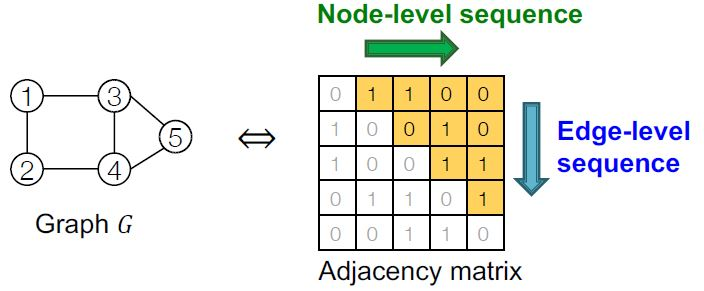
\includegraphics[width=0.85\linewidth]{notes/img/l10_p35_adj.JPG} \par
}

Recall in Section \ref{ss_621_basics} we raised the complexity/tractability issue of generating $n^2$ entries in the adjacency matrix given $n$ nodes. The solution we just presented does NOT solve this issue. It merely turned into a $\frac{n^2}{2}$ problem, not decreasing the magnitude of complexity. To solve this, we can claim that the node order (since we are generating node embeddings anyways and we are only given the number of nodes), that we are following BFS order. Let's use the $5$ node example again

\begin{enumerate}
    \item Starting at node $1$, we call this layer $0$
    
    \item Node $2, 3$ are generated. These connect to node $1$, therefore they are in layer $1$.
    
    \item Node $4$ does not connect to node $1$, so neighbour generation (think BFS) for layer $0$ is complete. Future nodes can only connect to $2, 3, 4$.
    
    \item When we generate edges for node $5$, node $1$ is no longer a candidate. 
    
    \item \textit{Suppose} that edge $3-4$ does not exist. Then neighbour generation for layer $1$ is complete, future nodes can only connect to $4, 5$.
\end{enumerate}{}

With BFS ordering, we only need to keep track of candidate nodes for $2$ layers, instead of the entire graph. This still does not solve the tractability issue, but reduces the average complexity to $O(n)$ rather than $O(n!)$. This enforced ordering also limits $O(n!)$ possible node orders to number of BFS orders possible for the given graph. 

With these in mind, the recurrent structure will be similar to a NLP-oriented structure that has a higher level RNN for words/tokens, then a lower level RNN that generate word embedding directly from characters. The following graph shows \textit{unrolled} RNN for node level and for edge level. Drawing an NLP analogy, the node level RNN provide ``context" for edge level RNN. The source of training loss is $0/1$ prediction generated from edge RNN. 
To speed up training, authors of the graph RNN paper used \textit{teacher-forcing} tecnique. That is, at training time, input to each RNN cell is the correct value from the previous step. See detailed explanation of teacher forcing \href{https://towardsdatascience.com/what-is-teacher-forcing-3da6217fed1c}{[here]}. Here, For each node, we use the \textit{correct} edge generation vector from its predecessor. For each edge, we use the \textit{correct} individual edge result from the previous edge. \textit{Done/EOS} signal from edge RNN is not necessary because we know exactly how many edges are supposed to be evaluated on. However, adding this additional signal provides more information to the RNN structure.

{
\centering
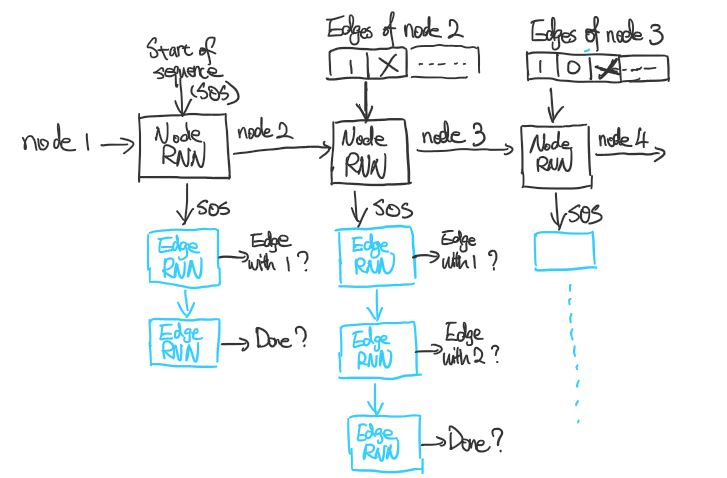
\includegraphics[width=0.85\linewidth]{notes/img/n6_rnn.JPG} \par
}

To evaluate the quality of generated graph, we can use various similarity metrics to compare the generated graph with some in-sample graphs. Similarity metrics can be based on graph statistics (Section \ref{s_2}) and visualization like the comparison below. This image shows that GraphRNN result resembles training samples, whereas baseline results are far from ideal.

{
\centering
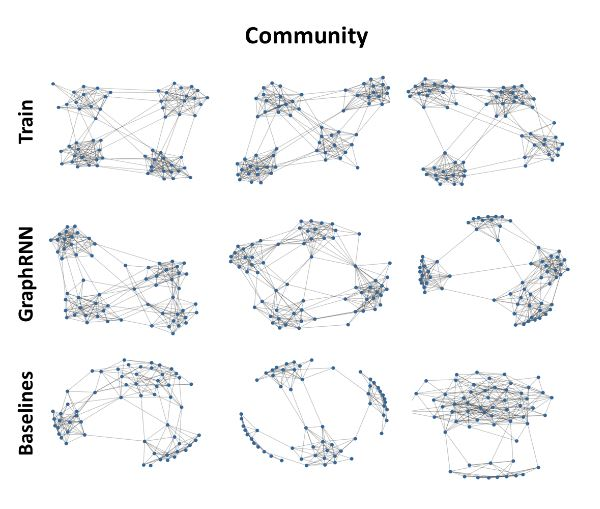
\includegraphics[width=0.5\linewidth]{notes/img/n6_compare.JPG} \par
}


Aside from these evaluation metrics, we can also setup the generation loss to include \textbf{goals} and \textbf{rules}. This is used for drug discovery where we want to generate valid chemicals and achieve certain chemical properties.

Since graph generation is an iterative process, reinforcement learning methods can also be employed, leading to \textit{Graph Convolutional Policy Network} (NIPS 2018) \href{https://arxiv.org/pdf/1806.02473.pdf}{[link]} where we setup the RL strategy to target metrics above.

At the moment, researchers are moving toward 3D graph generation where incorporation of positional information and/or representation of point cloud is open to discussion. Moreover, as we have discussed, complexity of generating graphs grow at a not-so-linear rate, thus generating large graphs can be a problem. Another layer of abstraction that have sub-structures as ``context" could be used like Kronecker graph generation method. We can also use neural methods for anomaly detection, such as unusual friend request, invalid chemicals, etc.

\subsection{Limitations of Graph Neural Network}

In the previous $2$ sections we discussed current development of graph neural networks, describing various state-of-the-art implementation for node classification and graph classification. Built on top of these methods, link prediction for content recommendation has also achieved incredible performance (NIPS 2018) \href{https://papers.nips.cc/paper/7763-link-prediction-based-on-graph-neural-networks}{[link]}. Despite these achievements, GNN methods have limitations. 

\subsubsection{Capturing Graph Structure}

Graph convolution is fundamentally a $1$-step operation that does not track whether a node has been visited like a path finding algorithm. Therefore, it has limited capability in recognizing difference in not-so-local structure until several layers of propagation. 

\paragraph{Detection of circular graph} Consider the following graph, where we are trying to check if the graph is circular. Starting a node $1$, we need $4$ rounds of information propagation before being able to verify that the graph is circular. With fewer than $4$ rounds, we have no way of knowing how node $4, 5, 6$ are connected.

{
\centering
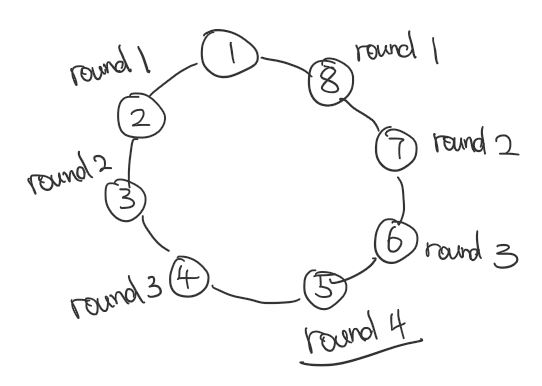
\includegraphics[width=0.5\linewidth]{notes/img/n6_circular.JPG} \par
}

\paragraph{Distinction between different neighbourhood setup} One possible neighbour aggregation function for vanilla graph convolution is taking the average of all neighbour nodes. Consider the $2$ following scenarios, where $X, Y$ are type of nodes. Clearly, simple average does not distinguish between having $2$ neighbours and $4$ neighbours, which could be important for many applications. Similarly, max pooling would lead to the same issue if embeddings of the same node class are the same. 

{
\centering
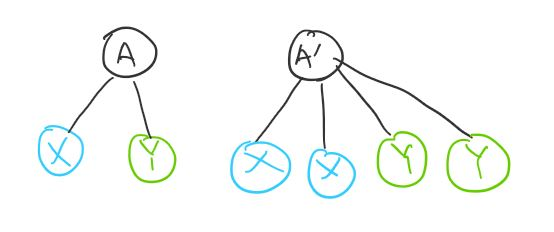
\includegraphics[width=0.5\linewidth]{notes/img/n6_avg.JPG} \par
}

To solve this issue, we have to design an injective neighbourhood aggregation function. Recall that \textit{injection} is the same as \textit{one-to-one correspondence}, meaning that for function $f$, $f(a) = f(b)$ if and only if $a=b$. With an injective neighbourhood aggregation function, $\sigma(f_{injective}(X, Y)) \neq \sigma(f_{injective}(X, X, Y))$.

It might sound strange but sum-pooling solves the above issue (ICLR 2019 \href{https://arxiv.org/pdf/1810.00826.pdf}{[link]}). And yes, sum-pooling does exactly what you think it does, just element-wise sum. Since we have $tanh$ as activation, we are not concerned with overflowing. $Tanh$ is an injective function because it is monotonically increasing. Also note that nested injective functions are also injective, thus convolution of multiple layers with sum-pooling remain injective, allowing difference in graph structures to be captured (still limited to number of layers, so ``detection of circular graph" type of issue cannot be solved). 

\paragraph{Weisfeiler-Lehman Isomorphism Test} The paper we just mentioned and its proposed sum-pooling method claimes to be comparable in power as Weisfeiler-Leham (WL) Isomorphism test, an iterative method that generates a canonical form for a graph. Unfortunately, WL is only surjective (If $f(a) \neq f(b)$ then $a \neq b$, but the other direction is not enforced). Here is the algorithm \href{https://www.davidbieber.com/post/2019-05-10-weisfeiler-lehman-isomorphism-test/}{[link]} for graph $G=(V, E)$ and neighbour function $N(v)$

\begin{enumerate}
    \item Assign unique representation $C_{0, v}$ to all $v \in V$
    
    \item Iterate the following steps for at least $|V|$ rounds
    
    \item For all $v\ in V$, at iteration $i$ (starting from $i=1$)
    
    \begin{enumerate}
        \item Get representations from previous step of all its neighbours, form a multiset (where duplicates are allowed, order does not matter) $\{C_{i-1, k} \forall k \in N(v)\}$
    
        \item Assign $C_{i, v} = Hash\Big( \{C_{i-1, k} \forall k \in N(v)\} \Big)$
    \end{enumerate}{}
\end{enumerate}{}

Suppose we want to compare $G_1(V_1, E_1)$ and $G_2(V_2, E_2)$, we would run WL on each of these graphs, thus have $multiset\{C_{|V_1|, v} \forall v \in V_1\}$ and $multiset\{C_{|V_2|, v} \forall v \in V_2\}$. If the generated multisets are different, then due to surjectivity of the algorithm, $G_1, G_2$ must not be isomorphic. Note that we can run the algorithm for both graphs in parallel, and terminate as soon as difference is observed at the end of each of the $|V|$ rounds.

From this algorithm, it is not hard to see that graphs that have similar local structure are likely going to lead to the same multiset output. The following shows one such case, where WL algorithm output is the same for $G_{skip}(11, 2)$ and $G_{skip}(11, 3)$.

{
\centering
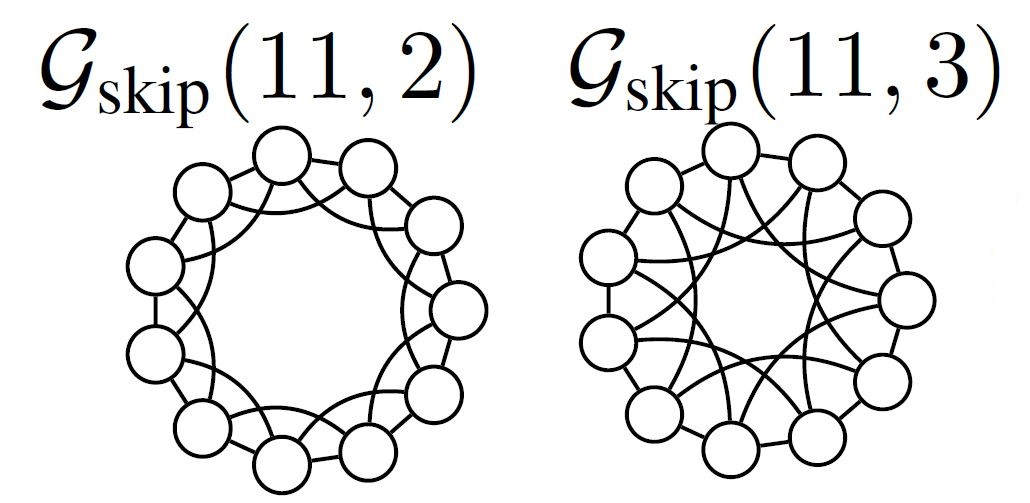
\includegraphics[width=0.5\linewidth]{notes/img/l18_p45_wl.JPG} \par
}

\subsubsection{Adversarial Attacks}

Graph neural network is a relatively new field. Model robustness has not been the top priority for researchers compared to the raw performance of GNN models. Theoretically, attack on GNN models aim to modify target/node features/classifications and/or the existence of edge between nodes. In the real world, we can classify direct attack (those that influence the target directly) as 

\begin{itemize}
    \item Modify the target's features. (Change website content generated based on node embedding)
    
    \item Add connections to the target. (Add fake followers and likes)
    
    \item Remove connections from the target. (Unfollow, untrust users)
\end{itemize}{}

For indirect attacks (the attacker modifies its own features/connections), the attacker can use its own characteristics to skew predictions made by GNN models to achieve its goal.

\begin{todo}
    Read https://arxiv.org/pdf/1805.07984.pdf then write a description of how adversarial attack is done on semi-supervised learning.
    
    Is it just a GNN derivation of https://arxiv.org/pdf/1412.6572.pdf?
\end{todo}{}

At the current stage, we can conclude that GNN methods are not safe to adversarial attack. Noticeable research in terms of model robustness include \href{https://arxiv.org/pdf/1905.03679.pdf}{[link]} and \href{http://pengcui.thumedialab.com/papers/RGCN.pdf}{[link]}, but these approaches have only been evaluated on standard datasets with vanilla GNN tasks. Effectiveness of these methods in the real-world has yet to be verified.

\end{document}